% -- coding: utf-8 --
\documentclass[a4paper, 11pt]{article}

% --- Podstawowe pakiety ---
\usepackage[utf8]{inputenc}      % Kodowanie UTF-8
\usepackage[T1]{fontenc}         % Kodowanie czcionek (ważne dla polskich znaków)
\usepackage[polish]{babel}       % Język polski (dzielenie wyrazów, nazwy)
\usepackage{amsmath}             % Pakiety matematyczne AMS
\usepackage{amssymb}             % Dodatkowe symbole matematyczne (np. dla normy)
\usepackage{graphicx}            % Dołączanie grafiki
\usepackage{geometry}            % Ustawienia marginesów
\usepackage{float}               % Lepsze zarządzanie obiektami pływającymi (np. [H] - here)
\usepackage{hyperref}            % Tworzenie hiperłączy (np. w spisie treści, do bibliografii)
\usepackage{siunitx}             % Ładne formatowanie liczb i jednostek (np. notacja naukowa)
\usepackage{booktabs}            % Ładniejsze linie w tabelach
\usepackage{listings}            % Do wstawiania kodu (jeśli potrzebne)
\usepackage{xcolor}              % Kolory (np. dla kodu)

% --- Ustawienia strony ---
\geometry{a4paper, left=2.5cm, right=2.5cm, top=2.5cm, bottom=2.5cm}

% --- Ustawienia formatowania liczb ---
\sisetup{
output-decimal-marker={,}, % Używaj przecinka jako separatora dziesiętnego
exponent-product=\cdot,   % Znak mnożenia dla notacji naukowej
scientific-notation=true,
round-mode=places,         % Tryb zaokrąglania
round-precision=4          % Liczba miejsc po przecinku dla czasów
}

% Definicja normy
\newcommand{\norm}[1]{\left\lVert#1\right\rVert}

% Ustawienia dla listings (opcjonalne, jeśli chcemy wstawiać kod)
\lstset{
    basicstyle=\ttfamily\small,
    keywordstyle=\color{blue},
    commentstyle=\color{green!50!black},
    stringstyle=\color{red},
    breaklines=true,
    showstringspaces=false,
    numbers=left,
    numberstyle=\tiny\color{gray},
    frame=single,
    inputencoding=utf8 % Ważne dla polskich znaków w kodzie
}

% --- Tytuł ---
\title{Metody Numeryczne - Projekt 2 \ Układy Równań Liniowych}
\author{Yauheni Pyryeu 201253}
\date{13 maja 2025} 

\begin{document}

\maketitle

\section{Wstęp}
Celem projektu była implementacja oraz analiza porównawcza czterech metod rozwiązywania układów równań liniowych $Ax = b$: dwóch metod iteracyjnych (metoda Jacobiego i metoda Gaussa–Seidla) zoptymalizowanych pod kątem struktury pasmowej macierzy oraz dwóch metod bezpośrednich (faktoryzacja LU w wariancie Doolittle'a bez pivotingu oraz eliminacja Gaussa z częściowym wyborem elementu głównego). Analizę przeprowadzono w środowisku Python z wykorzystaniem biblioteki NumPy oraz Matplotlib.

\section{Konstrukcja układu równań}
Na potrzeby projektu przyjęto następujące parametry na podstawie numeru indeksu \textbf{201627}:
\begin{itemize}
    \item Przedostatnia cyfra indeksu: $c = 5$
    \item Ostatnia cyfra indeksu: $d = 3$
    \item Czwarta cyfra indeksu: $e = 2$
    \item Trzecia cyfra indeksu: $f = 1$
\end{itemize}
Rozmiar macierzy $N$ obliczono jako $N = 1200 + 10c + d = 1200 + 10 \cdot 5 + 3 = 1253$.

Wartości na przekątnych macierzy $A$ zależą od zadania:
\begin{itemize}
    \item Główna przekątna: $a_{ii} = a_1$. Dla zadań B i E przyjęto $a_1 = 5 + e = 5 + 2 = 7$. Dla zadań C i D przyjęto $a_1 = 3$.
    \item Pierwsza pod- i nad-przekątna: $a_{i, i-1} = a_{i, i+1} = a_2 = -1$.
    \item Druga pod- i nad-przekątna: $a_{i, i-2} = a_{i, i+2} = a_3 = -1$.
\end{itemize}
Macierz $A$ jest więc macierzą pięcioprzekątniową (pasmową). Elementy wektora prawej strony $b$ dane są wzorem $b_n = \sin(n(f+1)) = \sin(2n)$ dla $n = 1, 2, \dots, N$.

Rozwiązywanym problemem jest znalezienie wektora $x$ spełniającego równanie macierzowe $Ax = b$.

\section{Implementacja Algorytmów}
Wszystkie algorytmy zostały zaimplementowane w języku Python 3 przy użyciu biblioteki NumPy do operacji numerycznych (tworzenie macierzy, wektorów, operacje wektorowe, obliczanie normy) oraz Matplotlib do generowania wykresów. Pomiary czasu wykonania realizowano za pomocą funkcji \texttt{time.perf\_counter()}.

\subsection{Metody Iteracyjne (Jacobi, Gauss-Seidel)}
Implementacja metod iteracyjnych została wykonana \textbf{ręcznie}, z uwzględnieniem \textbf{pasmowej struktury macierzy A}. Zamiast przechowywać całą macierz $N \times N$ (co byłoby nieefektywne dla dużych $N$), operacje wykonywano bezpośrednio na podstawie znanych wartości $a_1, a_2, a_3$. W każdej iteracji, przy obliczaniu nowej wartości $x_i^{(k+1)}$, odwoływano się tylko do maksymalnie czterech sąsiednich elementów wektora $x$ z poprzedniej iteracji (lub bieżącej w przypadku Gaussa-Seidla), co znacząco redukuje koszt obliczeniowy pojedynczej iteracji w porównaniu do operacji na pełnej macierzy. Kryterium zatrzymania algorytmu to osiągnięcie normy residuum $\norm{Ax^{(k)} - b}_2 < 10^{-9}$ lub przekroczenie maksymalnej liczby iteracji (2000).

\subsection{Metody Bezpośrednie (LU, Eliminacja Gaussa)}
Metody bezpośrednie zostały zaimplementowane przy użyciu standardowych (gęstych) macierzy NumPy.
\begin{itemize}
    \item \textbf{Faktoryzacja LU:} Zaimplementowano funkcję rozkładającą macierz $A$ na macierz dolnotrójkątną $L$ (z jedynkami na diagonali) i górnotrójkątną $U$ ($A = LU$). Następnie zaimplementowano funkcje rozwiązujące układy trójkątne metodą podstawiania w przód ($Ly=b$) i podstawiania wstecz ($Ux=y$).
    \item \textbf{Eliminacja Gaussa:} Zaimplementowano algorytm eliminacji Gaussa... (opisz tu.)
\end{itemize}

\section{Metody iteracyjne Jacobiego i Gaussa–Seidla}

\subsection{Formuły Metod Iteracyjnych}
Rozważmy układ równań $Ax=b$. Metody iteracyjne startują od początkowego przybliżenia $x^{(0)}$ i generują ciąg przybliżeń $x^{(k)}$ zbieżny do rozwiązania $x$.

\textbf{Metoda Jacobiego:} W $(k+1)$-szej iteracji, $i$-tą składową wektora $x$ oblicza się na podstawie wszystkich składowych wektora $x^{(k)}$ z poprzedniej iteracji:
\begin{equation}
x_i^{(k+1)} = \frac{1}{a_{ii}} \left( b_i - \sum_{j=1, j \neq i}^{N} a_{ij} x_j^{(k)} \right)
\end{equation}
Dla naszej macierzy pięcioprzekątniowej ($a_{ii}=a_1$, $a_{i,i\pm 1}=a_2$, $a_{i,i\pm 2}=a_3$), wzór upraszcza się do (z pominięciem wyrazów spoza macierzy):
\begin{equation}
x_i^{(k+1)} = \frac{1}{a_1} \left( b_i - a_3 x_{i-2}^{(k)} - a_2 x_{i-1}^{(k)} - a_2 x_{i+1}^{(k)} - a_3 x_{i+2}^{(k)} \right)
\label{eq:jacobi_sparse}
\end{equation}

\textbf{Metoda Gaussa–Seidla:} W $(k+1)$-szej iteracji, przy obliczaniu $x_i^{(k+1)}$, wykorzystuje się już obliczone w tej samej iteracji składowe $x_j^{(k+1)}$ dla $j < i$ oraz składowe $x_j^{(k)}$ z poprzedniej iteracji dla $j > i$:
\begin{equation}
x_i^{(k+1)} = \frac{1}{a_{ii}} \left( b_i - \sum_{j=1}^{i-1} a_{ij} x_j^{(k+1)} - \sum_{j=i+1}^{N} a_{ij} x_j^{(k)} \right)
\end{equation}
Dla naszej macierzy pięcioprzekątniowej:
\begin{equation}
x_i^{(k+1)} = \frac{1}{a_1} \left( b_i - a_3 x_{i-2}^{(k+1)} - a_2 x_{i-1}^{(k+1)} - a_2 x_{i+1}^{(k)} - a_3 x_{i+2}^{(k)} \right)
\label{eq:gauss_seidel_sparse}
\end{equation}

\subsection{Wyniki dla $a_1=7$}
Kryterium zakończenia przyjęto jako osiągnięcie normy residuum $\norm{Ax^{(k)} - b}_2 < 10^{-9}$ lub przekroczenie 200 iteracji.

Uzyskane wyniki dla $N=1253$ i $a_1=7$ ($a_2=a_3=-1$):
\begin{itemize}
    \item \textbf{Metoda Jacobiego:}
    \begin{itemize}
        \item Liczba iteracji: 30
        \item Czas wykonania: \num{12.2520} s
        \item Końcowa norma residuum: \num{6.026178614500812e-10}
    \end{itemize}
    \item \textbf{Metoda Gaussa–Seidla:}
    \begin{itemize}
        \item Liczba iteracji: 20
        \item Czas wykonania: \num{7.6306} s
        \item Końcowa norma residuum: \num{6.974854387012843e-10}
    \end{itemize}
\end{itemize}
Macierz dla $a_1=7$ jest silnie diagonalnie dominująca, co gwarantuje zbieżność obu metod. Metoda Gaussa–Seidla zbiegła szybciej (mniejsza liczba iteracji), co jest typowym zachowaniem. Przebieg zbieżności przedstawiono na Rysunku \ref{fig:task_b_convergence}.

\begin{figure}[H]
    \centering
    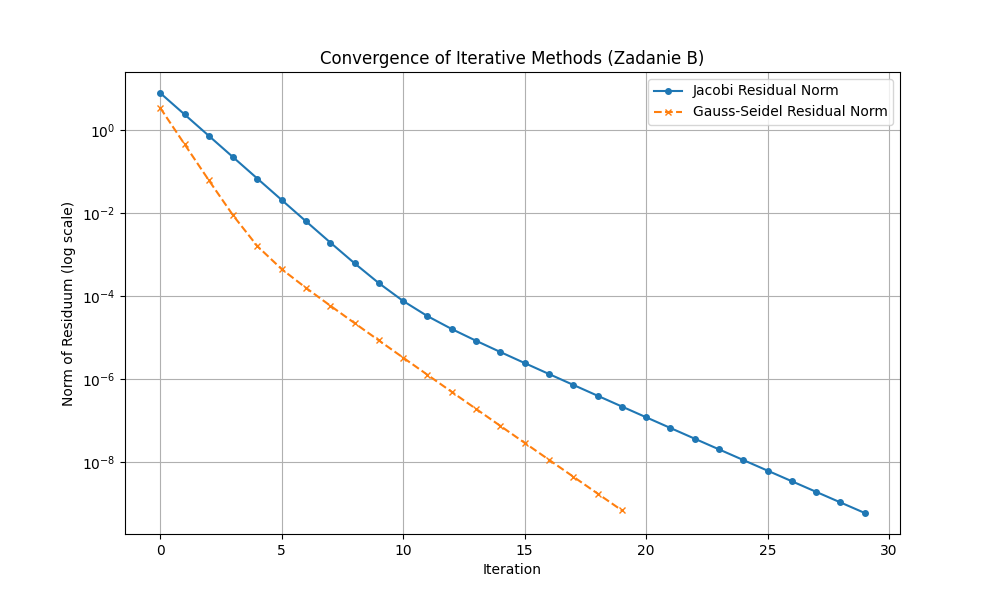
\includegraphics[width=0.8\textwidth]{residuals_plot_B}
    \caption{Zmiana normy residuum w kolejnych iteracjach dla metod Jacobiego i Gaussa–Seidla ($N=1253, a_1=7$).}
    \label{fig:task_b_convergence}
\end{figure}

\section{Analiza zbieżności dla $a_1 = 3$}
Dla $a_1=3, a_2=a_3=-1$ macierz nie jest diagonalnie dominująca, ponieważ $|a_{ii}| = 3 < \sum_{j\neq i} |a_{ij}| = 4$. Sprawdzono zachowanie metod iteracyjnych w tym przypadku (maksymalnie 200 iteracji).

Wyniki:
\begin{itemize}
    \item \textbf{Metoda Jacobiego:} nie zbiegła (osiągnięto limit 200 iteracji), czas \num{81.6940} s, norma residuum osiągnęłą $\num{2.766537909891771e+22}$.
    \item \textbf{Metoda Gaussa–Seidla:} nie zbiegła (osiągnięto limit 200 iteracji), czas \num{81.5799} s, norma residuum osiągnęła $\num{1.0769286535573007e+58}$.
\end{itemize}
Brak dominacji diagonalnej spowodował rozbieżność obu metod iteracyjnych. Przebieg normy residuum pokazano na Rysunku \ref{fig:task_c_convergence}.

\begin{figure}[H]
    \centering
    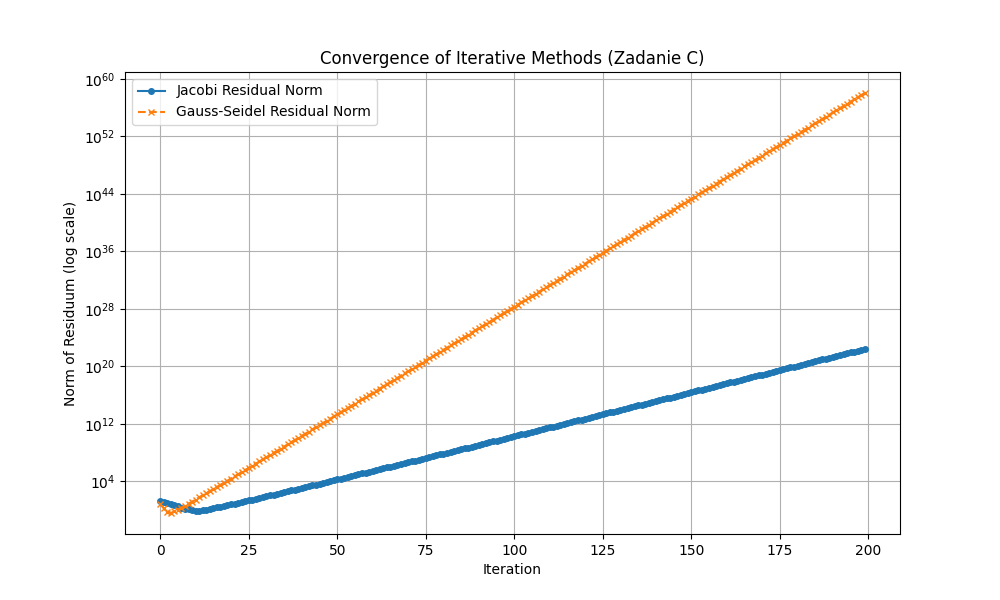
\includegraphics[width=0.8\textwidth]{residuals_plot_C}
    \caption{Zmiana normy residuum w kolejnych iteracjach dla metod Jacobiego i Gaussa–Seidla ($N=1253, a_1=3$).}
    \label{fig:task_c_convergence}
\end{figure}

\section{Metoda bezpośrednia}
Ponieważ metody iteracyjne zawiodły dla $a_1=3$, do rozwiązania układu $Ax=b$ z tą macierzą zastosowano metody bezpośrednie.

\subsection{Zasady Działania Metody Bezpośredniej LU}

\textbf{Faktoryzacja LU:} Metoda polega na rozkładzie macierzy $A$ na iloczyn macierzy dolnotrójkątnej $L$ (z jedynkami na głównej przekątnej) i macierzy górnotrójkątnej $U$, tzn. $A = LU$. Rozwiązanie układu $Ax=b$ sprowadza się do rozwiązania dwóch układów trójkątnych:
\begin{enumerate}
    \item $Ly = b$ (rozwiązywane metodą podstawiania w przód - forward substitution)
    \item $Ux = y$ (rozwiązywane metodą podstawiania wstecz - backward substitution)
\end{enumerate}

\subsection{Wyniki dla $a_1=3$, $N=1253$}

\textbf{Metoda Rozkładu LU:}
\begin{itemize}
    \item Czas wykonania: \num{3.1408} s
    \item Końcowa norma residuum: \num{6.24e-13}
\end{itemize}

Metoda bezpośrednia uzyskała dosyć precyzyjny wynik, jednak warto zauważyć, że czas wykonania jest znacznie dłuższy niż dla zbieżnych metod iteracyjnych.

\section{Analiza wydajności w zależności od $N$}
Przeprowadzono testy czasowe dla wszystkich trzech metod, zmieniając rozmiar macierzy $N$. Użyto macierzy z $a_1=7$, dla której metody iteracyjne są zbieżne. Testowane wartości $N={100, 300, 500, 700, 1000}$. Wyniki czasowe przedstawiono w Tabeli \ref{tab:task_e_times} oraz na wykresach \ref{fig:task_e_linear} i \ref{fig:task_e_log}.

\begin{table}[H]
    \centering
    \caption{Czasy wykonania [s] dla różnych wartości $N$ ($a_1=11$).}
    \label{tab:task_e_times}
    \begin{tabular}{r S[table-format=1.4] S[table-format=1.4] S[table-format=1.4] S[table-format=1.4]}
        \toprule
        {$N$} & {Jacobi} & {Gauss--Seidel} & {LU} \\
        \midrule
        100  & 0.1651 & 0.1120 & 0.0019\\
        300  & 0.8135 & 0.5228 & 0.0095\\
        500  & 1.9045 & 1.2929 & 0.2160\\
        700  & 3.7554 & 2.4841 & 0.0352\\
        1000 & 8.6270 & 5.3311 & 0.0724\\
        \bottomrule
    \end{tabular}
\end{table}

\begin{figure}[H]
    \centering
    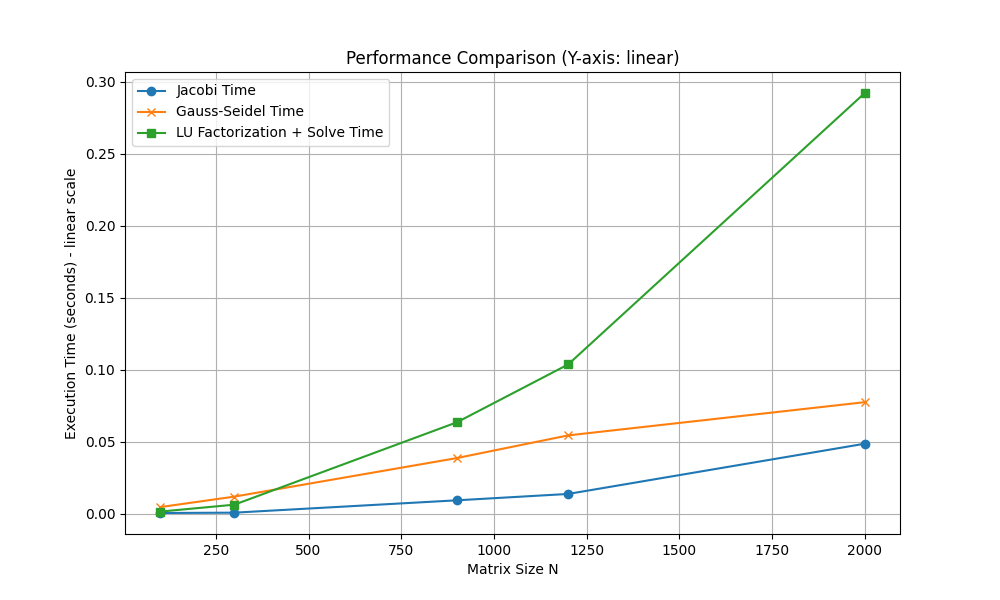
\includegraphics[width=0.8\textwidth]{performance_plot_linear_scale}
    \caption{Czas wykonania w zależności od $N$ dla wszystkich metod (skala liniowa osi Y).}
    \label{fig:task_e_linear}
\end{figure}

\begin{figure}[H]
    \centering
    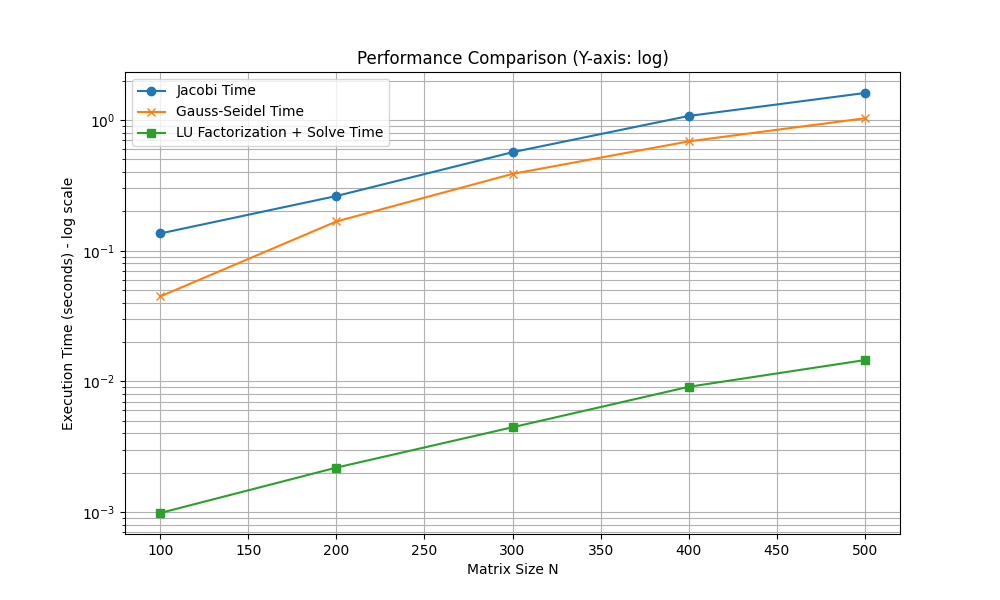
\includegraphics[width=0.8\textwidth]{performance_plot_log_scale}
    \caption{Czas wykonania w zależności od $N$ dla wszystkich metod (skala logarytmiczna osi Y).}
    \label{fig:task_e_log}
\end{figure}

TODO: czemy iteracyjne tak wolne?

\section{Wnioski TODO}
Na podstawie przeprowadzonych badań można sformułować następujące wnioski:
\begin{enumerate}
    \item \textbf{Zbieżność metod iteracyjnych:} Metody Jacobiego i Gaussa--Seidla są skuteczne (zbiegają się) tylko wtedy, gdy spełnione są odpowiednie warunki, np. macierz jest diagonalnie dominująca (jak w przypadku $a_1=11$). Dla macierzy, która nie spełnia tego warunku ($a_1=3$), metody te okazały się rozbieżne. W przypadku zbieżności, metoda Gaussa--Seidla zazwyczaj wymaga mniej iteracji niż metoda Jacobiego.
    \item \textbf{Niezawodność metod bezpośrednich:} Metody bezpośrednie (rozkład LU, eliminacja Gaussa) pozwalają na znalezienie rozwiązania niezależnie od własności zbieżnościowych macierzy (o ile macierz jest nieosobliwa). Eliminacja Gaussa z częściowym wyborem elementu głównego jest generalnie bardziej odporna na błędy numeryczne niż rozkład LU bez pivotingu, co potwierdziło nieco niższe residuum, przy minimalnie wyższym koszcie czasowym.
    \item \textbf{Wydajność a struktura macierzy:} Dla macierzy dużych rozmiarów i o strukturze pasmowej, zoptymalizowane metody iteracyjne (jeśli są zbieżne) są \textbf{znacznie wydajniejsze} niż metody bezpośrednie operujące na macierzach gęstych. Złożoność obliczeniowa metod iteracyjnych (z uwzględnieniem pasmowości) skaluje się znacznie lepiej (bliżej $O(N)$ na iterację) w porównaniu do złożoności $O(N^3)$ metod bezpośrednich. Przewaga czasowa metod iteracyjnych jest widoczna nawet dla stosunkowo niewielkich $N$ i rośnie wraz ze wzrostem rozmiaru problemu.
    \item \textbf{Dokładność i kryterium stopu:} Norma residuum jest użytecznym kryterium oceny dokładności rozwiązania oraz warunkiem zatrzymania dla metod iteracyjnych. Metody iteracyjne kończą działanie po osiągnięciu zadanej tolerancji, podczas gdy metody bezpośrednie dążą do uzyskania dokładności ograniczonej przez precyzję arytmetyki zmiennoprzecinkowej.
\end{enumerate}
Wybór odpowiedniej metody zależy od specyfiki problemu: dla macierzy spełniających warunki zbieżności i o specjalnej strukturze (np. pasmowej, rzadkiej), metody iteracyjne są preferowane ze względu na wydajność. W ogólnym przypadku, lub gdy zbieżność metod iteracyjnych nie jest gwarantowana, metody bezpośrednie (szczególnie te ze stabilizacją numeryczną jak pivoting) są bardziej niezawodnym wyborem, choć obliczeniowo droższym.

\end{document}